\documentclass{beamer}
\usepackage[serbian]{babel}
\usepackage{graphicx}
\usepackage{caption}
\usepackage{hyperref}
\usepackage{minted}
\usetheme{Madrid}

\definecolor{bluegreen}{RGB}{3, 166, 155}
\definecolor{pitchblack}{RGB}{0, 0, 0}
\definecolor{lightbeige}{RGB}{255, 251, 241}
\definecolor{mediumgray}{RGB}{183, 183, 183}

\setbeamercolor{author in head/foot}{bg=black,fg=white}
\setbeamercolor{date in head/foot}{bg=black,fg=white}
\setbeamercolor{title in head/foot}{bg=black,fg=white}
\setbeamercolor{page number in head/foot}{bg=black,fg=white}

\setbeamertemplate{headline}{%
\leavevmode%
  \hbox{%
    \begin{beamercolorbox}[wd=\paperwidth,ht=2.5ex,dp=1.125ex]{palette quaternary}%
    \insertsectionnavigationhorizontal{\paperwidth}{}{\hskip0pt plus1filll}
    \end{beamercolorbox}%
  }
}

\title{Akustični napad bočnog kanala nad tastaturama zasnovan na dubokom učenju}
\author{Momir Milutinović SV 39/2021}
\centering
\date{5. jul 2024.}
\begin{document}
\maketitle

\begin{frame}{Sadržaj}
\tableofcontents
\end{frame}

\section{Uvod}
\begin{frame}{Problem}
    \begin{itemize}
        \item Odrediti koji taster na tastaturi je pritsinut na osnovu zvuka pritiska tastera 
    \end{itemize}
    \begin{figure}
        \centering
        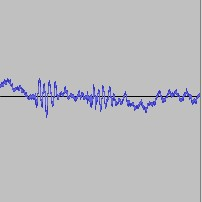
\includegraphics[scale=0.7]{KeystrokeSoundAudacity.jpg}
        \centering
        \captionsetup{justification=centering}
        \caption{Talasni oblik zvuka pritsika tastera}
        \label{fig:my_label}
    \end{figure}
\end{frame}

\section{Skup podataka}
\begin{frame}{Prikupljanje podataka}
    \begin{itemize}
        \item Svi tasteri za slova engleske su pritisnuti po 50 puta, različitim jačinama i menjajući prst kojim se pritiska taster
        \item Snimci su snimljeni ugrađenim mikrofonom laptopa
        \item Strani zvuci su dospeli u neke snimke
    \end{itemize}
    \begin{figure}
        \centering
        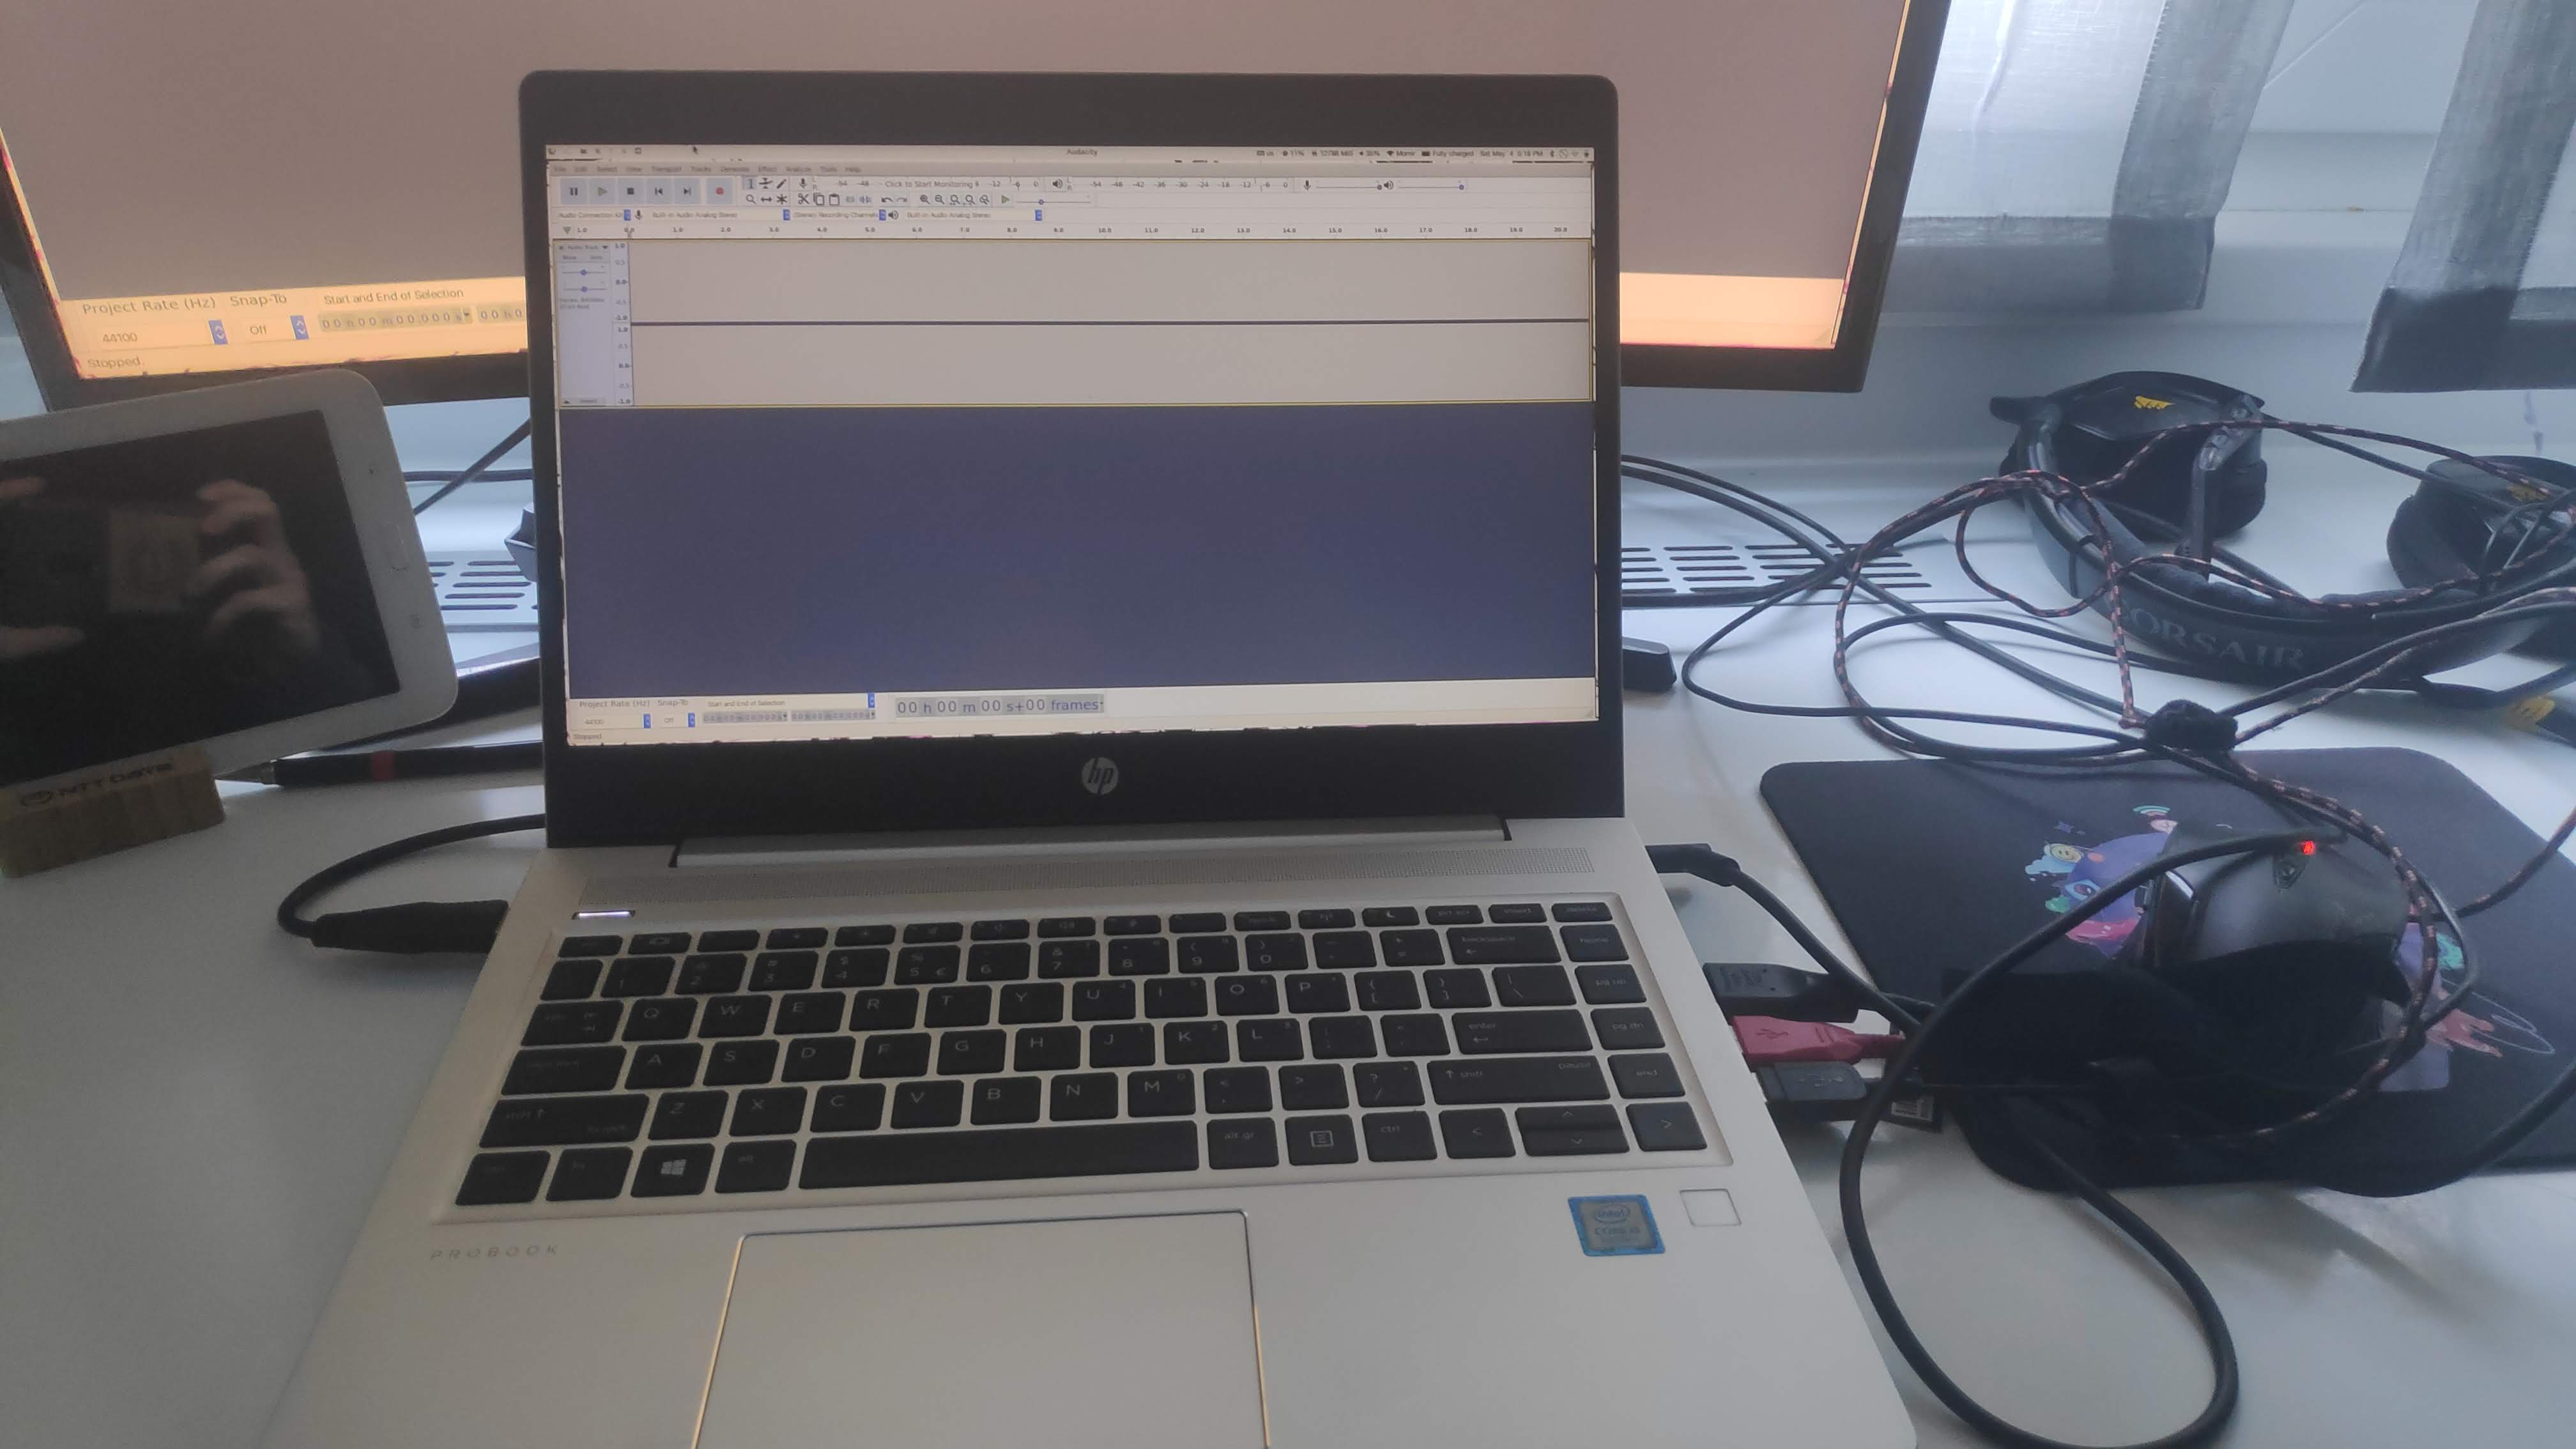
\includegraphics[scale=0.045]{Recording setup.jpg}
        \centering
        \captionsetup{justification=centering}
        \caption{Laptop koji je korišćen za snimanje}
        \label{fig:my_label}
    \end{figure}
\end{frame}

\begin{frame}{Izdvajanje pritisaka tastera}
    \begin{itemize}
        \item Postupak opisan u radu „A Practical Deep Learning-Based Acoustic Side
Channel Attack on Keyboards“
    \end{itemize}
    \begin{enumerate}
        \item Izračunava se energija signala primenom brze Furijeve transformacije i sumiranjem dobijenih koeficijenata
        \item Definiše se minimalna vrednost energije, koja ukazuje na prisustvo pritiska tastera
        \item Za svaki momenat u snimku gde je energija premašila prethodno defnisani prag se uzima isečak dužine 0.33 s koji počinje 0.1 s pre tog momenta
        \begin{itemize}
            \item Izolovani pritisci tastera se ne poklapaju
        \end{itemize}
        \item Minimalna vrednost energije, koja ukazuje na prisustvo pritiska tastera, se postepeno menja dok se ne izdvoji tačan broj pritisaka tastera
    \end{enumerate}
\end{frame}

\begin{frame}[fragile]{Algoritam za izdvajanje pritisaka tastera}
    \rule{\textwidth}{1pt}
    \scriptsize
    \begin{minted}{python}
    def nadji_prag(snimak, pocetni_prag, korak, trazeni_broj_pritisaka_tastera):
        trenutni_prag = pocetni_prag
        pritisci_tastera = izdvoj_pritiske_tastera(snimak, pocetni_prag)
        while len(pritisci_tastera) != trazeni_broj_pritisaka_tastera:
            if len(pritisci_tastera) > trazeni_broj_pritisaka_tastera:
                trenutni_prag += korak
            else:
                trenutni_prag -= korak
            korak = korak * 0.99
            pritisci_tastera = izdvoj_pritiske_tastera(snimak, trenutni_prag)
            
        return (pritisci_tastera, trenutni_prag) 
    \end{minted}
    \rule{\textwidth}{1pt}
\end{frame}

\begin{frame}{Izdvajanje osobina}
    \begin{itemize}
        \item Osobine snimaka se izdvajaju pravljenjem mel spektrograma
        \item x-osa predstavlja vreme, y-osa frekvenciju, a boja predstavlja amplitudu određene frekvencije u datom trenutku
        \item Korišćena je dužina prozora 1024 i 64 mel opsega
        \item Slike dimenzija 64x64 piksela
    \end{itemize}
    \begin{figure}
        \centering
        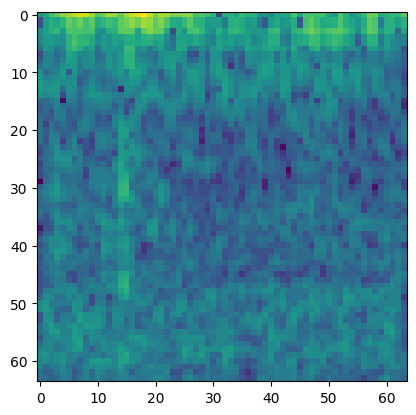
\includegraphics[scale=0.35]{MelSpectrogram.png}
        \centering
        \captionsetup{justification=centering}
        \caption{Mel spektrogram pritiska tastera}
        \label{fig:my_label}
    \end{figure}
\end{frame}
\begin{frame}{Augmentacija podataka}
    \begin{itemize}
        \item Nad spektrogramima u skupu za obuku je primenjena tehnika za augmentaciju podataka nazvana SpecAugment
        \begin{enumerate}
            \item Spektrogram se vremenski pomera za nasumični pomeraj do 30\% dužine spektrograma
            \item Maskiraju se 2 nasumična odsečka ose za vreme nasumičnih širina, koje mogu biti najviše 7 piksela (malo više od 10\% širine spektrograma)
            \begin{itemize}
                \item Maskirane vrednosti se zamenjuju prosečnom vrednošću spektrograma
            \end{itemize}
            \item Isto maskiranje se primenjuje i na osu za frekvenciju
        \end{enumerate}
    \item Augmentacija podataka za obuku se ponavlja u svakoj epohi
    \end{itemize}
\end{frame}
\begin{frame}{Primer spektrograma pre i nakon augmentacije podataka}
   \begin{columns}[t]
       \begin{column}{0.5\textwidth}
            \begin{figure}
                \centering
                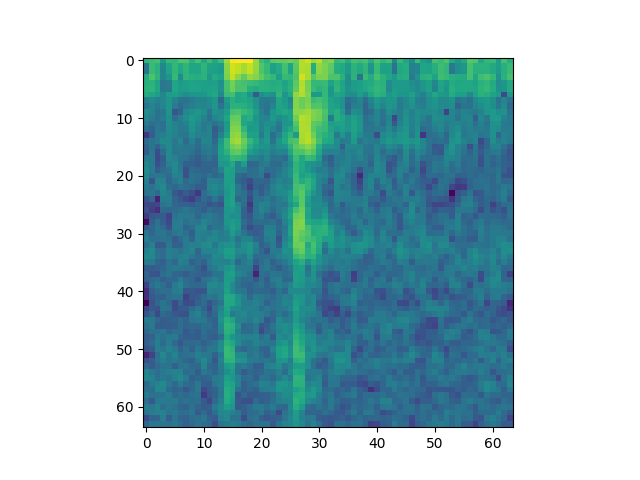
\includegraphics[scale=0.37]{SpectrogramBeforeAugment.png}
                \centering
                \captionsetup{justification=centering}
                \caption{Spektrogram pre primene SpecAugment}
                \label{fig:my_label}
            \end{figure}
       \end{column}
       \begin{column}{0.5\textwidth}
            \begin{figure}
                \centering
                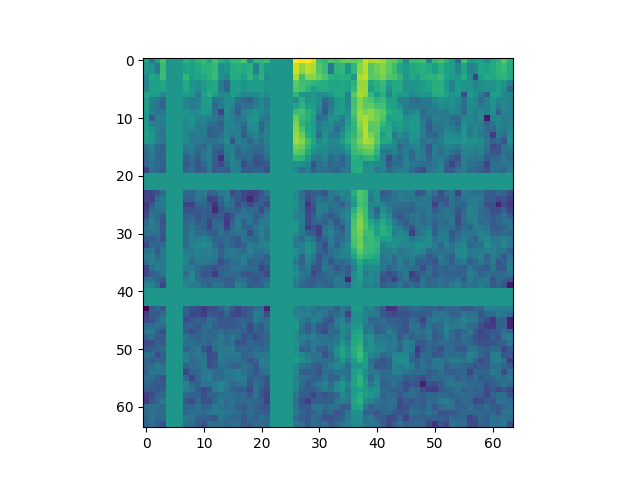
\includegraphics[scale=0.37]{SpectrogramAfterAugment.png}
                \centering
                \captionsetup{justification=centering}
                \caption{Spetkrogram nakon primene SpecAugment}
                \label{fig:my_label}
            \end{figure}
       \end{column}
   \end{columns}
\end{frame}
\section{Metod}
\begin{frame}{Arhitektura neurnoske mreže}
    \begin{itemize}
        \item Za arhitetkturu neuronske mreže za klasifikaciju spetkrograma je izabrana CoAtNet
        \item CoAtNet arhitektura je implmentirana u \textit{PyTorch} radnom okviru
    \end{itemize}
    \begin{figure}
        \centering
        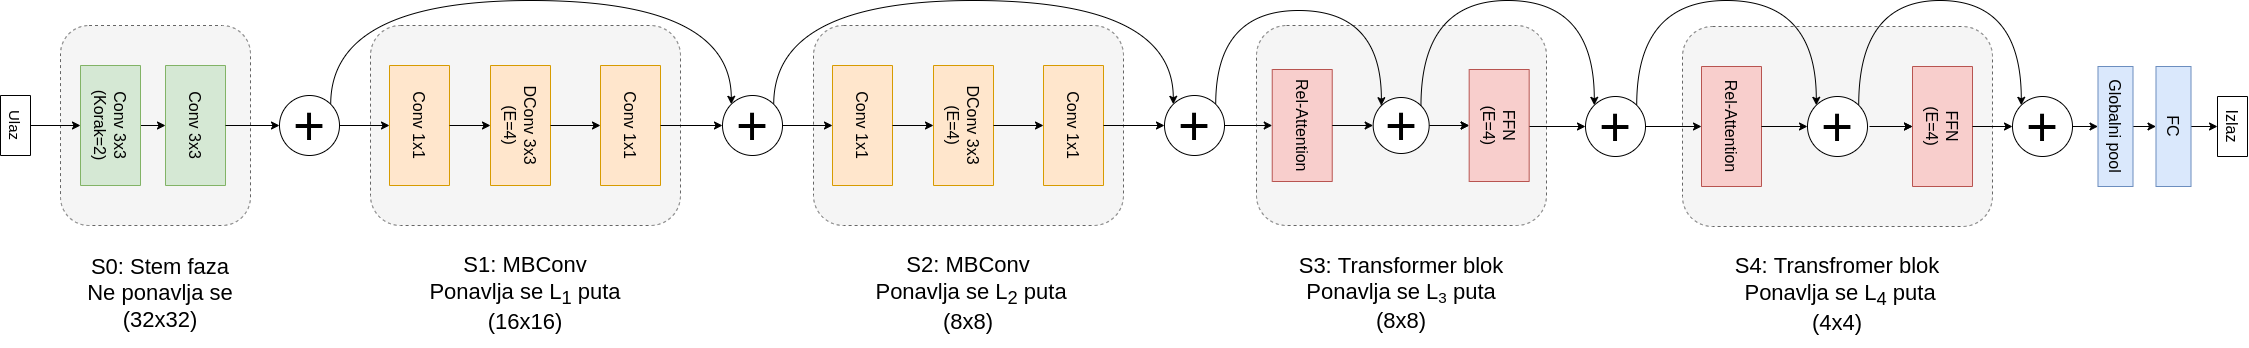
\includegraphics[scale=0.153]{CoAtNet.png}
        \centering
        \captionsetup{justification=centering}
        \caption{Dijagram CoAtNet arhitekture (Po uzoru na dijagram iz rada „CoAtNet: Marrying Convolution and Attention
for All Data Sizes“}
        \label{fig:my_label}
    \end{figure}
\end{frame}
\begin{frame}{Podela podataka}
\begin{itemize}
    \item Podaci su na podeljeni na skupove za obučavanje, validaciju i testiranje
    \item Odnos veličina skupova za treniranje, validaciju i testiranje je 60/20/20
    \item Podela je vršena na slučajan način 
\end{itemize}
\end{frame}
\begin{frame}{Izbor hiperparametara}
    \begin{itemize}
        \item Razmatrane su CoAtNet-0 i CoAtNet-1 varijante CoAtNet arhitekture
        \item FC i konvolutivni slojevi su inicijalizovani Kaiming inicijalizacijom
    \end{itemize}
    \begin{center}
        \begin{table}[h]
            \begin{tabular}{ l l } 
                 \hline
                 Hiperparametar & Vrednost \\
                 \hline
                 Broj epoha & 1100 \\
                 Veličina podskupa & 16 \\
                 Funkcija greške & \textit{Cross entropy} \\
                 Optimizacioni algoritam & \textit{AdamW} \\
                 Maksimalni korak učenja & $$5 \cdot 10^{-4}$$ \\
                 Minimalni korak učenja & $$10^{-6}$$ \\
                 Raspored koraka učenja & Linearan \\
                 Koeficijent smanjenja težina (eng. \textit{weight decay}) & 0.1 \\
                 \hline
            \end{tabular}
            \caption{Odabrane vrednosti hiperparametara}
            \label{tab:abc}
        \end{table}
    \end{center}
\end{frame}
\section{Rezultati i diskusija}
\begin{frame}{Rezultati}
    \begin{itemize}
        \item I CoAtNet-0 i CoAtNet-1 su postigle istu maksimalnu tačnost od 94.5\% na validacionom skupu 
        \item Izlažu se rezultati za CoAtNet-0 mrežu jer je ona manja
        \item Nad skupom za testiranje je dobijena tačnost od 91.8\%
    \end{itemize}
\end{frame}

\begin{frame}{Diskusija}
    \begin{itemize}
        \item Iz analize matrice konfuzije je primećeno da se netačno predviđeni tasteri uglavnom nalaze blizu ili pored tačnih tastera
        \item 12 pogrešnih predikcija su bile za 1 taster udaljene od tačnog tastera, od čega je njih 10 bilo levo ili desno
    \end{itemize}
    \begin{figure}
        \centering
        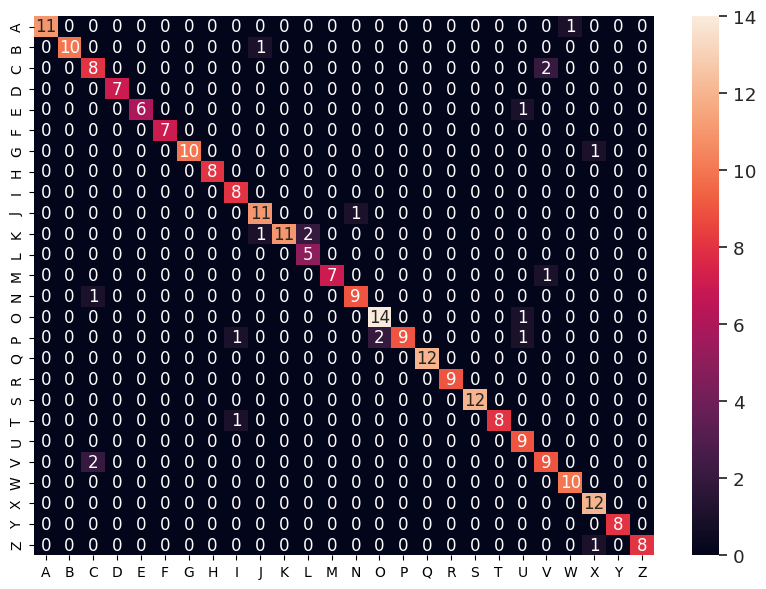
\includegraphics[scale=0.28]{ConfusionMatrix.png}
        \centering
        \captionsetup{justification=centering}
        \caption{Matrica konfuzije nad skupom za testiranje}
        \label{fig:my_label}
    \end{figure}
\end{frame}

\begin{frame}{Diskusija}
    \begin{itemize}
        \item Takođe možemo primetiti da je došlo do preprilagođavanja.
        \item Harrison et al. su istrenirali CoAtNet model koji postiže 95\% tačnosti nad snimcima sa telefona u blizini tastature
        \item Prethodno spomenuti istraživači su istrenirali model i nad snimcima iz Zoom aplikacije sa najmanjim podešavnjima smanjenja šuma i dobili su 93\% tačnosti
        \item Akinbi et al. su napravili ConvMixer model koji ima tačnost od 92.4\% nad snimcima sa telefona
        \item Moji rezultati ne predstavljaju poboljšanje nad postojećim, ali greške ispoljavaju iste obrasce koji su uočili Harrison et al.
    \end{itemize}
\end{frame}

\section{Zaključak}
\begin{frame}{Zaključak}
\begin{itemize}
    \item Obučena je efiksana mreža za klasifikaciju zvukova tastera na tastaturi
    \item Duboko učenje se pokazalo kao efikasna metoda za izvršavanje napada bočnog kanala nad tastaturama
    \item Rezultati Harrison et al. su uspešno reprodukovani
\end{itemize}
\end{frame}

\begin{frame}[t]{Literatura}
    \begin{enumerate}
        \item Harrison, J., Toreini, E., & Mehrnezhad, M. (2023, July). A practical deep learning-based acoustic side channel attack on keyboards. In 2023 IEEE European Symposium on Security and Privacy Workshops (EuroS&PW) (pp. 270-280). IEEE.
        \item Dai, Z., Liu, H., Le, Q. V., & Tan, M. (2021). Coatnet: Marrying convolution and attention for all data sizes. Advances in neural information processing systems, 34, 3965-3977.
        \item Taheritajar, A., Harris, Z. M., & Rahaeimehr, R. (2023). A Survey on Acoustic Side Channel Attacks on Keyboards. arXiv preprint arXiv:2309.11012.
        \item Akinbi, A., Deniz, E., Ismael, A. M., Rashid, Z. N., & Sengur, A. (2023). Password-sniffing acoustic keylogger using machine learning. Available at SSRN 4431909.
    \end{enumerate}
\end{frame}
\begin{frame}[t]{Literatura}
    \begin{enumerate}
        \setcounter{enumi}{4}
        \item https://www.kaggle.com/code/anastasiialobanova/my-coatnet
        \item https://github.com/xmu-xiaoma666/External-Attention-pytorch/blob/master/model/attention/CoAtNet.py
        \item https://m0nads.wordpress.com/tag/self-attention/
        \item https://github.com/chinhsuanwu/coatnet-pytorch/blob/master/coatnet.py
    \end{enumerate}
\end{frame}

\end{document}
